\section{Even Data Placement Algorithm}
\label{sec:algorithm}

In this section, we propose the {\em Even Data Placement (EDP)} algorithm, a
polynomial-time greedy algorithm that aims to efficiently identify a
near-optimal data placement solution to Problem~\ref{problem:gap} in
Section~\ref{subsec:p_form}.  We also extend the EDP algorithm for the
heterogeneous setting. 

\subsection{Main Idea}

%As described in Section~\ref{subsec:p_form}, using brute-force algorithm to find the solution to Problem~(\ref{eq:normal_problem}) imposes untolerable latency on the write path.
%The greedy heuristic can simplify the complexity, and it distributes each unique chunks of the $i$-th file to the $j$-th node with minimum number of existing chunks, and the complexity is linear.
%By existing chunks, it means duplicate chunks plus previously assigned unique chunks of the same file in the distribution batch.
%As there are multiple files and each node should be distributed equal number of unique chunks in a batch distribution, the greedy algorithm alone does not guarantee an accurate solution.
%We provide an example on why greedy heuristic fails in our problem model when we illustrate our EDP algorithm in Figure~\ref{fig:edp_demo}.

%The EDP algorithm extends the greedy heurisic. 
The EDP algorithm builds on two procedures: \textsc{Distribute} and
\textsc{Swap}.  The \textsc{Distribute} procedure attempts to identify a node
to place each chunk of a batch such that the increase in the summation of the
read balance gaps is minimum.  If more than one node satisfies this criterion,
then we place the chunk at the node where the previous chunk of the same file
resides so as to keep the chunks of the same file together.  The \textsc{Swap}
procedure inspects the placement decision of \textsc{Distribute} and attempts
to swap the chunk positions of different file pairs to see if the summation of
the read balance gaps can be further reduced.  There are two types of unique
chunks in a batch that can be swapped: (i) {\em non-shared chunk}, which
appears in exactly one file in the batch, and (ii) {\em shared chunk}, which
appears in more than one file in the batch.  Since swapping shared chunks may
affect the chunk distributions of multiple files, for simplicity, we only
consider the swapping of non-shared chunks.  Note that the EDP algorithm only
operates on the chunk positions rather than the chunks, and does not incur any
actual I/O.   


%If this still does not resolve the tied situation, we choose the next node in a round-robin fashion. 

%For each of the $t$ files in a batch, the EDP algorithm first follows the greedy heuristic to distribute the unique chunks, which we call the \textsc{Distribute} step, and, then, attempts all possible swaps of distribution decisions on unique chunks of current file with those of previously processed files in the batch, which we call the \textsc{Swap} step.
%Note that all the swaps involve only in-memory operations on temporary decisions on where to distribute the unique chunks, and do not incur any actual I/Os.
%The existence of two types of unique chunks: i) \emph{non-shared chunk} that appears in only one of the files in the batch; ii) \emph{shared chunk} that is shared by multiple files, in a batch complicates the swapping step as swapping shared chunks affects chunk distribution of multiple files.
%Therefore, EDP considers swapping of non-shared chunks only.
%If there are multiple nodes with equal smallest number of existing blocks, apart from placing blocks evenly for each file in one segment, we also seek to sequentially place blocks so as to optimize file access performance for each storage node. 
%If this still does not resolve the tied situation, we choose the next node in a round-robin fashion. 

%Finally, EDP outputs the distribution decision as a list of mapping from unique chunk ID to storage node ID, and sends this result to client for file data transmission.

%We require that data blocks from each file are placed sequentially in each storage node. Also, data blocks in one segment are required to be placed file by file, i.e., blocks from File~$i$ are always placed in front of File~$j$, where $0 \leq i < j <t$. Based on the above two instructions, we use the following three steps to determine the balanced data placement for files in one segment:

%The \textit{EDP} algorithm can be summerized by 2 main steps:
%\begin{enumerate}
%\item [(1)]
%\emph{File-by-file Greedy Distribution:} \textit{EDP} first greedily distributes unique blocks of each file to fill the distribution buffer.
%For each file, we example the problem of allocating a given total storage budget, i.e., the amount of unique blocks in the file, in a distributed storage system with data deduplication. We greedily place it to maximize its file distribution index. Note the previously stored duplicate blocks should also be taken into account.
%\item [(2)]
%\emph{Inter-file Adjustment:} To further improve the overall min-max metric, \textit{EDP} tentatively swaps the distribution decisions on unique blocks between each pair of storage nodes for different file pairs. 
%Upon all data blocks of a file being placed, we greedily exchange the its storage allocation with that of previously storage files so as to maximize the segment fairness distribution index.
%\item [(3)]
%\emph{Block placement:} After distributed storage allocations for all files are determined, we first determine the exact placement positions for all blocks sequentially. We then consider the exchange the position of blocks that are contained in the following files with that of unique blocks in one file, so as to further increase the segment fairness distribution index.
%\end{enumerate}

\subsection{Algorithm Details}

Algorithm~\ref{alg:edp} shows the pseudo-code of the EDP algorithm.  It takes
the following inputs: 
(i) $N$, the number of storage nodes;
(ii) $C$, the number of unique chunks to be placed in each node ;
(iii) $t$, the number of files in a batch; 
(iv) $\mathbf{U} = (U_i|1\le i \le t)$, a vector where each entry is the
number of unique chunks of each file;
(v) $\mathbf{d} = (d_{i,j} | 1 \le i \le t, 1 \le j \le N)$, a vector where
each entry is the number of duplicate chunks of each of the $t$ files on each
of the $N$ nodes; and 
(vi) $\mathbf{F} = (F_l | 1 \le l \le N\times C)$, a vector where each entry
is the list of files in the batch that share the unique chunk $l$. 
It outputs $\mathbf{u} = (u_{i,j}|1\le i \le t, 1\le j \le N)$, a vector where
each entry indicates the number of unique chunks of each of the $t$ files to
place in each of the $N$ nodes.

For each file, the EDP algorithm first calls \textsc{Distribute} (Line~6) to
assign unique chunks of each file $i$ to the storage nodes.  It also records
the current objective value (Line~$7$).  It then calls \textsc{Swap} to
attempt to swap the chunk positions of the current file with those of the
previous files to further reduce the objective value (Lines~8-10).

In \textsc{Distribute}, for each unique chunk (Line~15), EDP tentatively
assigns it to each of the $N$ nodes, and finds the node that minimizes the
change of $G_i$ if the chunk is assigned to it (Line~16).  If there are
multiple nodes that have the same minimal change of $G_i$, EDP assigns the
chunk to the same node as the previous chunk.  Then EDP increments the number
of unique chunks for the current file on that node by one (Line~17).  For
other files in the batch that share this unique chunk, EDP increments the
number of duplicate chunks of each such file on the selected node by one
(Lines~18-20).  Finally, EDP decrements the allowable number of chunks 
on the selected node by one (Line~21).

In \textsc{Swap}, EDP inspects possible swaps of placement decisions for a
given pair of files denoted by indices $i$ and $i'$ between each possible pair
of nodes denoted by indices $j$ and $j'$ (Line~25).  EDP focuses on the
non-shared chunks, and counts the number of non-shared chunks of files~$i$ and
$i'$ on nodes~$j$ and $j'$ as $m_{i,j}$ and $m_{i',j'}$, respectively
(Lines~26-27).  Then EDP tries all possible numbers of unique chunks,
denoted by $z$, from one up to $\min(m_{i,j},m_{i',j'})$, to swap (Line~28).
For each $z$, EDP records the revised objective value if $z$ non-shared chunks
of files~$i$ and $i'$ are swapped between nodes~$j$ and $j'$ (Line~29).  EDP
picks $z$ that minimizes the objective value as $z^*$ (Line~31).  If the
objective value after swapping is smaller than that without swapping, the swap
decision will be made (Lines~32-36).
%If the swapping is executed, the distribution decisions on the swapped chunks will be updated accordingly(Line~$34$).

\begin{algorithm}[H]
\begin{small}
%\begin{multicols}{2}
\begin{algorithmic}[1]
%\Require \par
%$t$: number of files in the batch;\par
%$N$: number of available storage nodes;\par
%$C$: number of unique chunks to distribute to each node in a batch;\par
%$\mathbf{U}$: $\{U_i | 1 \le i \le t\}$ ;\par
%$\mathbf{F}$: $\{\mathbf{F}_l |$ list of files that share the unique chunk $l$, $1 \le l \le N\times C\}$;\par
%$\mathbf{d}$: $\{d_{i,j} | 1 \le i \le t, 1 \le j \le N \}$.
%\Ensure \par
%$P_{i,j}$: ID of the node where the $j$-th chunk of the file $i$ is assigned;\par
%$\mathbf{u}$: $\{u_{i,j} | 1 \le i \le t, 1 \le j \le N \}$.

\Function{EDP}{$t,N,C,\mathbf{U},\mathbf{F},\mathbf{d}$}
\caption{Even Data Placement Algorithm}
\label{alg:edp}
%\State $\mathbf{P}_{i,j}$ $\leftarrow$ -1, $i \in \{0,\dots,t-1\}, j \in \{0,\dots,\mathcal{U}_i-1\}$
\State $u_{i,j}$ $\leftarrow$ $0$, $1 \le i \le t, 1 \le j \le N$
\State $C_j \leftarrow C, 1 \le j \le N$
\State $T \leftarrow 0$
\For{$i$ = 1 to $t$}
  %\State\Comment{File-by-file greedy distribtion}
  \State \Call{Distribute}{$i,T,\mathbf{U},\mathbf{C},\mathbf{F},\mathbf{u},\mathbf{d}$}

  \State $S \leftarrow$ $\sum_{k=1}^{i} G_k$

  %\State\Comment{Inter-file Adjustment}
  \For{$i'$ = 1 to $i-1$}
	\State \Call{Swap}{$i,i',\mathbf{u},\mathbf{d},S$}     
   \EndFor
   \State $T \leftarrow T + U_i$
\EndFor

%\State \Return $\SP$
\EndFunction
\Function{Distribute}{$i,T,\mathbf{U},\mathbf{C},\mathbf{F},\mathbf{u},\mathbf{d}$}
\For{$l$ = 1 to $U_i$}
     %\For{$m$ = 1 to $N$}
     %\State $I_k = G(\{u_{i,1},\dots,u_{i,k}+1,\dots,u_{i,N}\},d_i), 1\leq k \leq N ~and~C_k > 0$ 
     %\State $k^*$ = argmin$_{k}$ $I_k$
     %\State 
     %\EndFor
     \State $j^* \leftarrow $ ID of node that minimizes change of $G_i$
     \State $u_{i,j^*} \leftarrow u_{i,j^*} + 1$
     \For{\textbf{each} $i' \in \mathbf{F}_{l+T}$}
     \State $d_{i',j^*} \leftarrow d_{i',j^*}+1$
     \EndFor
     \State $C_{j^*} \leftarrow C_{j^*} - 1$
\EndFor
\EndFunction

\Function{Swap}{$i,i',\mathbf{u},\mathbf{d},S$}
\For{each storage node pair $(j, j')$}
	%\State $\mathbf{l}_{i,x} \leftarrow$ all local unique chunks of file $i$ on node $x$
	%\State $\mathbf{l}_{j,y} \leftarrow$ all local unique chunks of file $j$ on node $y$
	\State $m_{i,j} \!\leftarrow\!$ number of non-shared chunks of file $i$ on node $j$
	\State $m_{i',j'} \!\leftarrow\!$ \mbox{number of non-shared chunks of
		file $i'$ on node $j'$}
	%\State\Comment{Start tentative swapping}
        \For{$z$ = 1 to min($m_{i,j}$, $m_{i',j'}$)}
       	  %\State Swap z chunks of file $i$,$i'$ between nodes $j$,$j'$
            \State $S_{z} \leftarrow$ $\sum_{k=1}^{i} G_k$, if $z$ non-shared
			chunks of 
			\Statex\hspace{0.5in} files $i$ and $i'$ are swapped between nodes~$j$ and $j'$ 
            %\State Resume z chunks of file $i$,$j$ between nodes $x$,$y$
          \EndFor
         \State $z^* \leftarrow$ argmin$_{1 \le z \le \min(m_{i,j},m_{i',j'})}$ $S_{z}$
	%\State $z^* \leftarrow $ the number of non-shared chunks to swap that minimizes $\sum_{l=1}^{i} G_l$, $1 \le z^* \le \min{num_{i,j},num_{i',j'}}$
	%\State\Comment{Execute the best swapping}
          \If{$S_{z^*} < S$}
	  \State Swap $z^*$ chunks of file $i$,$i'$ between nodes $j$,$j'$
	  \State{Update placement of the swapped chunks}
	   %  \For{$1 \leq k < z^*$}
	%	\State $P_{i,l_{i,x,k}} \leftarrow y, P_{j,l_{j,y,k}} \leftarrow x$
	 %    \EndFor
           \State $S \leftarrow S_{z^*}$
	\EndIf
      \EndFor
\EndFunction
\end{algorithmic}
%\end{multicols}
\end{small}
\end{algorithm}

\subsection{Example} 

Figure~\ref{fig:edp_demo} shows an illustrative
example with two files in a batch to be stored on a system of three nodes
using (3,2) erasure coding.  We set $C = 2$.  As shown in
Figure~\ref{fig:edp_demo_files}, suppose that file~1 has four unique chunks
and has $(d_{1,1},d_{1,2},d_{1,3}) = (2,0,1)$, and that file~2 has four unique
chunks and has $(d_{2,1},d_{2,2},d_{2,3}) = (1,1,0)$.

To balance the placement of chunks of file~1, EDP places two unique chunks on 
nodes~2 and 3, as shown in Figure~\ref{fig:edp_demo_file0}.
%Note that, when both node 2 and 3 have 1 existing chunk of file 1 after chunk A is assigned to node 2, chunk B is assigned to node 2 for better sequentiality.
As both chunks A and C are shared by file~2, EDP updates 
$(d_{2,1},d_{2,2},d_{2,3}) = (1,2,1)$.  For file~2, 
\textsc{Distribute} can only assign its two unique chunks to node~1.  At the
end of \textsc{Distribute}, the distributions of unique and duplicate chunks
of files~1 and 2 are: 
$(u_{1,1}+d_{1,1},u_{1,2}+d_{1,2},u_{1,3}+d_{1,3}) = (2,2,3)$ and
$(u_{2,1}+d_{2,1},u_{2,2}+d_{2,2},u_{2,3}+d_{2,3}) = (3,2,1)$, respectively.

\textsc{Swap} now tries swapping the positions of non-shared chunks of 
files~1 and file~2.  Before \textsc{Swap}, the objective value (i.e., the sum
of read balance gaps of files~1 and 2) is 
$(1 - \frac{7/3}{3}) + (1 - \frac{2}{3})= \frac{5}{9}$. 
Suppose now we try to swap chunks E and D, as shown in
Figure~\ref{fig:edp_demo_swap}.  The revised distributions of unique and
duplicate chunks of files~1 and 2 will become:
$(u_{1,1}+d_{1,1},u_{1,2}+d_{1,2},u_{1,3}+d_{1,3}) = (3,2,2)$ and
$(u_{2,1}+d_{2,1},u_{2,2}+d_{2,2},u_{2,3}+d_{2,3}) = (2,2,2)$, respectively.
The objective value can reduce to 
$(1 - \frac{7/3}{3}) + (1 - \frac{2}{2}) = \frac{2}{9}$.  This shows that
swapping of chunks~E and D can achieve better read balance. 

\begin{figure}[H]
\centering
\vspace{-10pt}
\subfigure[Example of files: assuming $( d_{1,1}, d_{1,2}, d_{1,3}) =
(2,0,1)$ and $(d_{2,1}, d_{2,2}, d_{2,3}) = (1,1,0)$. ]{
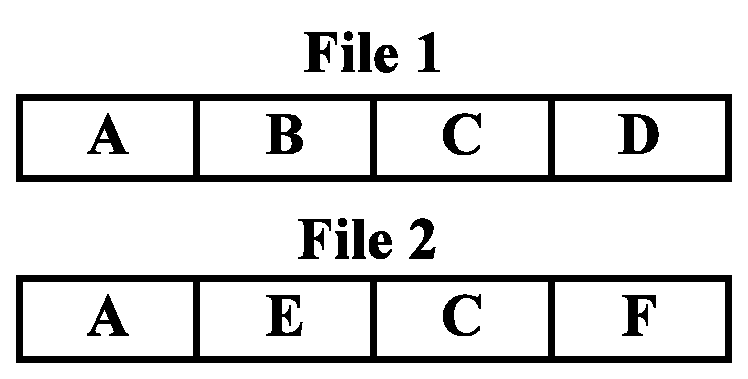
\includegraphics[width=3in]{edp_demo_files.eps}
\label{fig:edp_demo_files}
}
\\
\hspace{4pt}
\subfigure[ Greedy placement of File~1: $(u_{1,1}, u_{1,2}, u_{1,3}) = (0,2,2)$; $(d_{2,1}, d_{2,2}, d_{2,3}) = (1,2,1)$. ]{
\includegraphics[width=3in]{edp_demo_greedy.eps}
\label{fig:edp_demo_file0}
}
\\
\subfigure[ Greedy placement of File 2. $(u_{2,1}, u_{2,2}, u_{2,3})=(2,0,0)$. ]{
%The overall distribution of file 1 and 2 are (2,2,3) and (3,2,1). ]{
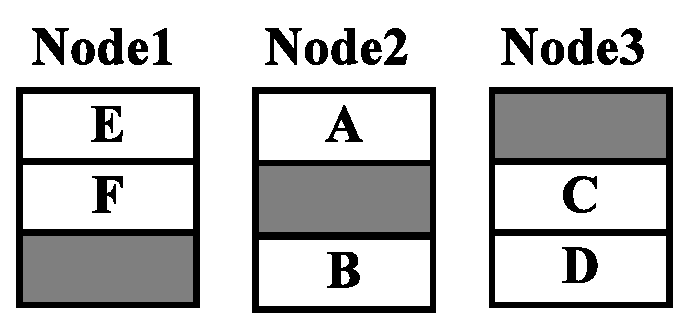
\includegraphics[width=3in]{edp_demo_file1.eps}
\label{fig:edp_demo_file1}
}
\\
\hspace{4pt}
\subfigure[ Swapping E and D. ]{
\includegraphics[width=3in]{edp_demo_swap.eps}
\label{fig:edp_demo_swap}
}
\caption{\Large Illustration of the EDP algorithm for two files, where $N = 3$, 
	$C = 2$, $(n,k) = (3,2)$. }
\label{fig:edp_demo}
\vspace{-6pt}
\end{figure}


%The basic idea of our EDP algorithm is as follows. For each File~$i$ in a segment, EDP firstly maximizes its fairness distribution index (Steps 3-13), and then tries to reduce the segment fairness distribution index via exchanging storage allocations between File~$i$ and File~$j(0 \leq j<i)$ (Steps 16-29). Finally, EDP determines the exact block placements for each data block in the segment (Steps 32-48). 


%Take Figure~\ref{fig:example} as an example for illustration. We firstly consider placing file~0. As there is no data in the storage system, blocks $A$, $B$ $C$, $D$ will be placed evenly across Node~0 to Node~3. We continue to place file~1. As block $A$ from file~0 has already been stored, it will be ignored. And then $E$ and $F$ of $G$ will be placed in Node~4, Node~1 and Node~2, respectively. We place blocks of file~2, file~3 and file~4 in the similar way. The adjustment process gives no benefit to the segment index. The block placement is shown in Figure~\ref{fig:example_conv3}. 

\subsection{Complexity Analysis}
\label{subsubsec:complexity}

We now derive the worst-case complexity of the EDP algorithm.  For each chunk
of file~$i$, \textsc{Distribute} inspects all $N$ storage nodes and a list of
up to $t$ files.  Thus, the complexity of \textsc{Distribute} on processing 
file~$i$ is $\mathcal{O}(U_i(N+t))$.
%Thus, the complexity of \textsc{GreedyDistribution} is $\mathcal{O}(cN^2)$. 
%Actually, in \textsc{GreedyDistribution}, the more expensive task is to update duplicate distribution for files that share the current chunk. 
%According to definition of $\mathbf{ld}$, its worset-case size if $cnt$. 
%Thus, the worst-case complexity of updating duplicate distributions is $\mathcal{O}(c^2n^2t)$. 
On the other hand, the \textsc{Swap} procedure scans possible swaps for 
file~$i$ and each of previous $i-1$ files between every pair of nodes,
and one swapping can involve up to $C$ chunks.  Thus, the complexity for
\textsc{Swap} to process file~$i$ is $\mathcal{O}((i-1)CN^2)$.  Hence, the
overall complexity of EDP when processing $t$ files is 
$\mathcal{O}(\max\{\sum_{i=1}^t U_i(N+t), \sum_{i=1}^t (i-1)CN^2\}) =
\mathcal{O}(CN^2t^2)$, which is in polynomial time. 

%, which is much more efficient than brute-force algorithm (see
		%Section~\ref{subsec:p_form}).

%\textbf{About error-bound between greedy+swapping algorithm (EDP) and theoretical optimal result(OPT)} Theory not ready, but, based on simulation results, gap between EDP and OPT is neglictable (very little for Linux dataset, zero for SVN and Synthetic).

\subsection{Extensions}
\label{subsec:cedp}

We consider two extensions, which account for heterogeneity and variable-size
chunks. 

{\bf Heterogeneity:} Algorithm~\ref{alg:edp} can be modified slightly to adapt
to the heterogeneous scenario, and we call it the
%where nodes have heterogeneous download costs, and, as the modified algorithm
%aims at balancing download cost of a file among the storage nodes, we call it
\textit{Cost-based Even Data Placement (CEDP)} algorithm.  According to
Section~\ref{subsec:heterogeneity}, the read balance gap is computed based on
the node weights. 
%we suppose the static
%download cost for all the storage nodes are kept in array $\mathbf{w}$, where
%$w_{j}$ indicates the download cost of node $j$, $j \in \{1,\dots,N\}$. 
For CEDP, the only change to EDP is to modify the calculation of the read
balance gap in Lines~7, 16, and 29 of Algorithm~\ref{alg:edp}.  Other steps
remain the same. 
%into $G'$, which enables
%between distribution of chunks and the theoretical even distribution for each
%file.  Therefore, we need to modify the function of read balance level on
%Line~$7$, $16$ and $29$ of Algorithm~\ref{alg:edp} into $G'$, which enables
%CEDP to dynamically distribute unique chunks to balance total download cost
%on each node for all the files in the buffer.

{\bf Variable-size chunking:} We can extend Algorithm~\ref{alg:edp} to support
variable-size chunking by calculating the read balance gap as a function of
the number of bytes (rather than the number of chunks).  We still write $C$
unique chunks to each node to maintain storage balance, yet we modify
$\mathbf{u}$ and $\mathbf{d}$ to indicate the numbers of unique and duplicate
bytes, respectively.  Specifically, let $\mathbf{L} = \{L_{i,j}|1\le i\le t,
1\le j \le U_i\}$, where $L_{i,j}$ is the length of chunk $j$ of file $i$.  In
\textsc{Distribute}, we modify Lines~17 and 19 as $u_{i,j^*} \leftarrow
u_{i,j^*} + L_{i,l}$ and $d_{i',j^*} \leftarrow d_{i',j^*} + L_{i,l}$,
respectively.  Also, in \textsc{Swap}, we modify Lines~29 and 33 to update
$u_{i,j}$ and $u_{i',j'}$ by the number of bytes of unique chunks that are
swapped.  We also modify the objective functions in Equations~(\ref{eq:gap})
and (\ref{eqn:hete_min_max}) in terms of numbers of bytes. 

%In the \textsc{Distribute} step, when we assign a unique chunk $l$ of the $i$-th 
%file to the $j^*$-th node, we should increment $u_{i,j^*}$ by the length of the chunk
% , i.e. $L_{i,l}$. For other file, $i'$, that shares this unique chunk, we should 
%update its $d_{i',j^*}$ by $L_{i,l}$ as well. To achieve this, we modify Lines~17 and 
%19 of Algorithm~\ref{alg:edp} into $u_{i,j^*} \leftarrow u_{i,j^*} + L_{i,l}$ and 
%$d_{i',j^*} \leftarrow d_{i',j^*} + L_{i,l}$, respectively.
%In the \textsc{Swap} step, when we swap the assignments of unique chunks of the $i$-th 
%and $i'$-th files between the $j$-th and $j'$-th nodes at Lines~29 and 33, we only 
%need to modify the $u_{i,j}$ and $u_{i',j'}$ based on lengths of the unique chunks that 
%are swapped. Note that the Formulas~(\ref{eq:gap}) and (\ref{eqn:hete_min_max}) to calculate 
%read balance gap remain the same.

%To get the heterogeneous version of our even data placement algorithm (i.e.,CEDP), we merely substitute Equation~\ref{eq:problem_form2} and Equation~\ref{eq:problem_form4} which are used to compute the fairness distribution index of $\SA$ and $\SP$ in Algorithm~\ref{alg:edp} with Equation~\ref{eq:problem_form112} and Equation~\ref{eq:problem_form5}, respectively. We expect CEDP can remain robust in maintaining recovery efficiency in heterogeneous settings...

%\begin{figure}[!ht]
%\centering
%\subfigure[Sequential block placements in one segment]{
%\includegraphics[width=1.6in]{edp.eps}
%\label{fig:example_conv3}
%}
%\subfigure[Block placements after adjustment]{
%\includegraphics[width=1.6in]{edp1.eps}
%\label{fig:example_conv4}
%}
%\caption{An illustrative example for even data placement algorithm.}
%\label{fig:example2}
%\end{figure}

%\subsection{Extension to Balancing Degraded Reads}
%\label{subsec:algo_degraded}

%\begin{algorithm}[t]
%\begin{algorithmic}[1]
%\caption{Degraded Reads Balancing Algorithm}
%\label{alg:degraded}
%\Require \par
%t: number of files;\par
%$\mathcal{U}_i$: number of unique blocks for file $i$; \par
%$\mathbf{pd}_{i,j,k}$: number of parities on node $k$ that are protecting blocks on node $j$ of file $i$; \par
%$\mathbf{u}_{i,j}$: number of unique blocks of file $i$ assigned to node $j$.
%$\mathbf{r2p}_{i,j}$: map the entry on $j$-th row of node $i$ to its parity block's node id.
%\Ensure \par
%$\mathbf{p}_{i,j}$: ID of node where the parity block of the $j$-th block of file $i$ resides.
%\Function{DegradedBalance}{$t$,$\mathcal{U}$,$\mathbf{u},\mathbf{pd},\mathbf{r2p},\mathbf{p}$}
%\State $\mathbf{p}_{i,j} \leftarrow -1, i\in\{0,\dots,t-1\}, j\in\{0,\dots,\mathcal{U}_i-1\}$
%\For{$i$ = 0 to $t-1$}
%    \State $block\_id \leftarrow 0$
%    \For{$j$ = 0 to $n-1$}
%         \For{$k$ = 0 to $\mathbf{u}_{i,j}$}
%	     \State $n^* \leftarrow$ ID of the node whose has the minimum $\mathbf{pd}_{i,j,n}, n\in\{0,\dots,n-1\}$, excluding $j$
%	     \State $\mathbf{p}_{i,block\_id} \leftarrow n^*$
%	     \State $\mathbf{pd}_{i,j,n^*} \leftarrow \mathbf{pd}_{i,j,n^*} + 1$
%	     \State $block\_id \leftarrow 1+block\_id$
%     	 \EndFor
%    \EndFor
%\EndFor
%\EndFunction
%\end{algorithmic}
%\end{algorithm}

%To further improve degraded reads performance, we propose Algorithm~\ref{alg:degraded} that balances number of parity chunks that are read from each survival node in case of node failure.
%The degraded reads balancing algorithm is based on ouptut of Algorithm~\ref{alg:edp}, and should be invoked after the even placement algorithm is done on current distribution buffer.
%The first three inputs of the algorithm are statistics on files, unique blocks and parity blocks, and they can be collected as the buffer is being filled.
%As for the output, the algorithm will decide on where each unique block's parity block should be distributed, and, after erasure coding, the client can distribute the parity block based on this information.

%For each unique block of a file, its destination node is detemined by EDP algorithm, and the degraded reads balancing algorithm associates the block to a stripe, whose parity block resides on the node with minimum number of parity blocks that protect blocks of the same file on current block's destination node. (Line~$5$)
%Then, the algorithm add this decision to ouput array (Line~$6$), updates the statistics on parity blocks (Line~$7$), and moves on to next unique block.

%The Algorithm~\ref{alg:degraded} is of linear complexity, and should have neglictable effects on the write path.
